\startcontents[localtoc]
\printcontents[localtoc]{}{0}{\subsection*{Contents}\setcounter{tocdepth}{2}}



\phantomsection
\addcontentsline{toc}{section}{Generate sample data}
\subsubsection*{Generate sample data}



A random numbers with normal probability distribution function will be generated into input data \texttt{DI.y.v}. Next a drift will be added.

\begin{lstlisting}
DI = [];
DI.y.v = 1.5 + 3.*randn(1, 1e3);
DI.y.v = DI.y.v + [1:1:1e3]./100;
\end{lstlisting}


Lets suppose a sampling frequency is 1 Hz. The algorithm will generate all possible tau values automatically.

\begin{lstlisting}
DI.fs.v = 1;
\end{lstlisting}


\phantomsection
\addcontentsline{toc}{section}{Call algorithm}
\subsubsection*{Call algorithm}



Use QWTB to apply algorithm \texttt{ADEV} to data \texttt{DI}.

\begin{lstlisting}
DO = qwtb('ADEV', DI);
\end{lstlisting}
\begin{lstlisting}[language={},xleftmargin=5pt,frame=none]
QWTB: no uncertainty calculation

\end{lstlisting}


\phantomsection
\addcontentsline{toc}{section}{Display results}
\subsubsection*{Display results}



Log log figure is the best to see allan deviation results:

\begin{lstlisting}
figure; hold on
loglog(DO.tau.v, DO.adev.v, '-b')
loglog(DO.tau.v, DO.adev.v + DO.adev.u, '-k')
loglog(DO.tau.v, DO.adev.v - DO.adev.u, '-k')
xlabel('\tau (sec)');
ylabel('\sigma_y(\tau)');
title(['period = ' num2str(1/DI.fs.v)]);
grid('on'); hold off
\end{lstlisting}
\begin{center}
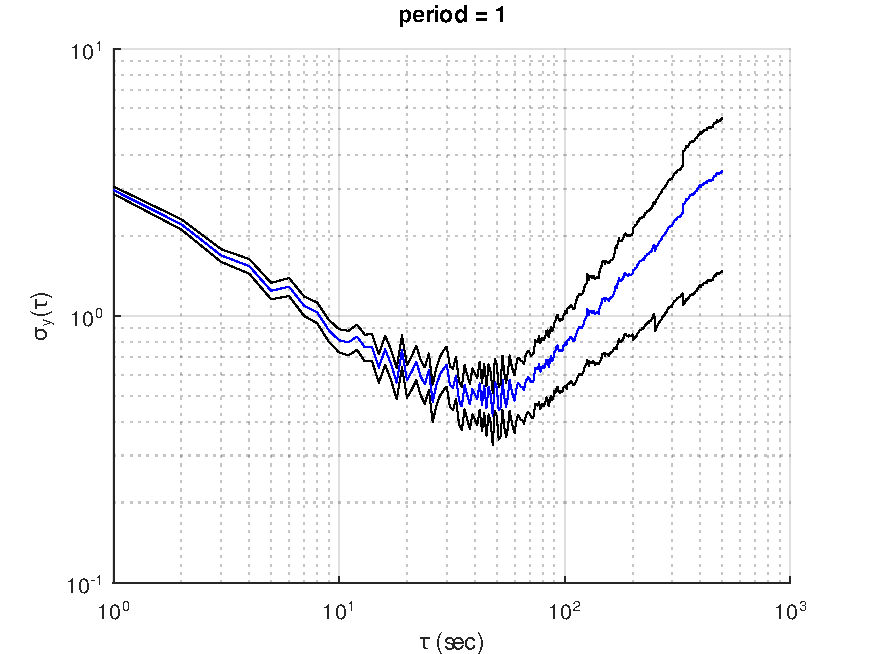
\includegraphics[width=0.7\textwidth]{algs_examples_published/ADEV_alg_example-1.pdf}
\end{center}


\stopcontents[localtoc]
